% Options for packages loaded elsewhere
\PassOptionsToPackage{unicode}{hyperref}
\PassOptionsToPackage{hyphens}{url}
%
\documentclass[
]{book}
\usepackage{lmodern}
\usepackage{amssymb,amsmath}
\usepackage{ifxetex,ifluatex}
\ifnum 0\ifxetex 1\fi\ifluatex 1\fi=0 % if pdftex
  \usepackage[T1]{fontenc}
  \usepackage[utf8]{inputenc}
  \usepackage{textcomp} % provide euro and other symbols
\else % if luatex or xetex
  \usepackage{unicode-math}
  \defaultfontfeatures{Scale=MatchLowercase}
  \defaultfontfeatures[\rmfamily]{Ligatures=TeX,Scale=1}
\fi
% Use upquote if available, for straight quotes in verbatim environments
\IfFileExists{upquote.sty}{\usepackage{upquote}}{}
\IfFileExists{microtype.sty}{% use microtype if available
  \usepackage[]{microtype}
  \UseMicrotypeSet[protrusion]{basicmath} % disable protrusion for tt fonts
}{}
\makeatletter
\@ifundefined{KOMAClassName}{% if non-KOMA class
  \IfFileExists{parskip.sty}{%
    \usepackage{parskip}
  }{% else
    \setlength{\parindent}{0pt}
    \setlength{\parskip}{6pt plus 2pt minus 1pt}}
}{% if KOMA class
  \KOMAoptions{parskip=half}}
\makeatother
\usepackage{xcolor}
\IfFileExists{xurl.sty}{\usepackage{xurl}}{} % add URL line breaks if available
\IfFileExists{bookmark.sty}{\usepackage{bookmark}}{\usepackage{hyperref}}
\hypersetup{
  pdftitle={Empowerment in Agriculture},
  pdfauthor={Teresia Mrema Buza},
  hidelinks,
  pdfcreator={LaTeX via pandoc}}
\urlstyle{same} % disable monospaced font for URLs
\usepackage{color}
\usepackage{fancyvrb}
\newcommand{\VerbBar}{|}
\newcommand{\VERB}{\Verb[commandchars=\\\{\}]}
\DefineVerbatimEnvironment{Highlighting}{Verbatim}{commandchars=\\\{\}}
% Add ',fontsize=\small' for more characters per line
\usepackage{framed}
\definecolor{shadecolor}{RGB}{248,248,248}
\newenvironment{Shaded}{\begin{snugshade}}{\end{snugshade}}
\newcommand{\AlertTok}[1]{\textcolor[rgb]{0.94,0.16,0.16}{#1}}
\newcommand{\AnnotationTok}[1]{\textcolor[rgb]{0.56,0.35,0.01}{\textbf{\textit{#1}}}}
\newcommand{\AttributeTok}[1]{\textcolor[rgb]{0.77,0.63,0.00}{#1}}
\newcommand{\BaseNTok}[1]{\textcolor[rgb]{0.00,0.00,0.81}{#1}}
\newcommand{\BuiltInTok}[1]{#1}
\newcommand{\CharTok}[1]{\textcolor[rgb]{0.31,0.60,0.02}{#1}}
\newcommand{\CommentTok}[1]{\textcolor[rgb]{0.56,0.35,0.01}{\textit{#1}}}
\newcommand{\CommentVarTok}[1]{\textcolor[rgb]{0.56,0.35,0.01}{\textbf{\textit{#1}}}}
\newcommand{\ConstantTok}[1]{\textcolor[rgb]{0.00,0.00,0.00}{#1}}
\newcommand{\ControlFlowTok}[1]{\textcolor[rgb]{0.13,0.29,0.53}{\textbf{#1}}}
\newcommand{\DataTypeTok}[1]{\textcolor[rgb]{0.13,0.29,0.53}{#1}}
\newcommand{\DecValTok}[1]{\textcolor[rgb]{0.00,0.00,0.81}{#1}}
\newcommand{\DocumentationTok}[1]{\textcolor[rgb]{0.56,0.35,0.01}{\textbf{\textit{#1}}}}
\newcommand{\ErrorTok}[1]{\textcolor[rgb]{0.64,0.00,0.00}{\textbf{#1}}}
\newcommand{\ExtensionTok}[1]{#1}
\newcommand{\FloatTok}[1]{\textcolor[rgb]{0.00,0.00,0.81}{#1}}
\newcommand{\FunctionTok}[1]{\textcolor[rgb]{0.00,0.00,0.00}{#1}}
\newcommand{\ImportTok}[1]{#1}
\newcommand{\InformationTok}[1]{\textcolor[rgb]{0.56,0.35,0.01}{\textbf{\textit{#1}}}}
\newcommand{\KeywordTok}[1]{\textcolor[rgb]{0.13,0.29,0.53}{\textbf{#1}}}
\newcommand{\NormalTok}[1]{#1}
\newcommand{\OperatorTok}[1]{\textcolor[rgb]{0.81,0.36,0.00}{\textbf{#1}}}
\newcommand{\OtherTok}[1]{\textcolor[rgb]{0.56,0.35,0.01}{#1}}
\newcommand{\PreprocessorTok}[1]{\textcolor[rgb]{0.56,0.35,0.01}{\textit{#1}}}
\newcommand{\RegionMarkerTok}[1]{#1}
\newcommand{\SpecialCharTok}[1]{\textcolor[rgb]{0.00,0.00,0.00}{#1}}
\newcommand{\SpecialStringTok}[1]{\textcolor[rgb]{0.31,0.60,0.02}{#1}}
\newcommand{\StringTok}[1]{\textcolor[rgb]{0.31,0.60,0.02}{#1}}
\newcommand{\VariableTok}[1]{\textcolor[rgb]{0.00,0.00,0.00}{#1}}
\newcommand{\VerbatimStringTok}[1]{\textcolor[rgb]{0.31,0.60,0.02}{#1}}
\newcommand{\WarningTok}[1]{\textcolor[rgb]{0.56,0.35,0.01}{\textbf{\textit{#1}}}}
\usepackage{longtable,booktabs}
% Correct order of tables after \paragraph or \subparagraph
\usepackage{etoolbox}
\makeatletter
\patchcmd\longtable{\par}{\if@noskipsec\mbox{}\fi\par}{}{}
\makeatother
% Allow footnotes in longtable head/foot
\IfFileExists{footnotehyper.sty}{\usepackage{footnotehyper}}{\usepackage{footnote}}
\makesavenoteenv{longtable}
\usepackage{graphicx}
\makeatletter
\def\maxwidth{\ifdim\Gin@nat@width>\linewidth\linewidth\else\Gin@nat@width\fi}
\def\maxheight{\ifdim\Gin@nat@height>\textheight\textheight\else\Gin@nat@height\fi}
\makeatother
% Scale images if necessary, so that they will not overflow the page
% margins by default, and it is still possible to overwrite the defaults
% using explicit options in \includegraphics[width, height, ...]{}
\setkeys{Gin}{width=\maxwidth,height=\maxheight,keepaspectratio}
% Set default figure placement to htbp
\makeatletter
\def\fps@figure{htbp}
\makeatother
\setlength{\emergencystretch}{3em} % prevent overfull lines
\providecommand{\tightlist}{%
  \setlength{\itemsep}{0pt}\setlength{\parskip}{0pt}}
\setcounter{secnumdepth}{5}
\usepackage{booktabs}
\usepackage{amsthm}
\makeatletter
\def\thm@space@setup{%
  \thm@preskip=8pt plus 2pt minus 4pt
  \thm@postskip=\thm@preskip
}
\makeatother
\usepackage[]{natbib}
\bibliographystyle{apalike}

\title{Empowerment in Agriculture}
\author{Teresia Mrema Buza}
\date{Updated: 2020-10-12 23:01:57}

\begin{document}
\maketitle

{
\setcounter{tocdepth}{1}
\tableofcontents
}
\hypertarget{prerequisites}{%
\chapter{Prerequisites}\label{prerequisites}}

This book is intendes for providing empowerment model models translated from literature into R code. For the most part we use M0 model developed previously for global poverty assessment \citep{Alkire2011}.

\hypertarget{methodology}{%
\section{Methodology}\label{methodology}}

\begin{tmbinfo}
\begin{enumerate}
\def\labelenumi{\arabic{enumi}.}
\tightlist
\item
  Method 1 focuses on the percentage of empowered women and adequacies
  among the disempowered.
\item
  Method 2 focuses on the percentage of disempowered women and the
  percentage of domains in which they lack adequate achievements.
\end{enumerate}

\begin{quote}
Method 2 is commonly used as it is consistent with the M0 measurement
(Alkire and Foster 2011).
\end{quote}

\begin{itemize}
\tightlist
\item
  The disempowerment cut-off (k=20\% ) is the percentage of weighted
  inadequacies a woman must have to be considered disempowered.
\item
  If ciw \textless= k the score is replaced by 0.
\item
  Any existing inadequacies are not considered in the ``Disempowered
  headcounts.
\item
  Now the matrix has new column \texttt{ciwk} that contains censored
  inadequacy score.
\end{itemize}
\end{tmbinfo}

This is a \emph{sample} book written in \textbf{Markdown}. You can use anything that Pandoc's Markdown supports, e.g., a math equation \(a^2 + b^2 = c^2\).

The \textbf{bookdown} package can be installed from CRAN or Github:

\begin{Shaded}
\begin{Highlighting}[]
\KeywordTok{install.packages}\NormalTok{(}\StringTok{"bookdown"}\NormalTok{)}
\CommentTok{\# or the development version}
\CommentTok{\# devtools::install\_github("rstudio/bookdown")}
\end{Highlighting}
\end{Shaded}

Remember each Rmd file contains one and only one chapter, and a chapter is defined by the first-level heading \texttt{\#}.

To compile this example to PDF, you need XeLaTeX. You are recommended to install TinyTeX (which includes XeLaTeX): \url{https://yihui.name/tinytex/}.

\hypertarget{intro}{%
\chapter{Introduction}\label{intro}}

You can label chapter and section titles using \texttt{\{\#label\}} after them, e.g., we can reference Chapter \ref{intro}. If you do not manually label them, there will be automatic labels anyway, e.g., Chapter \ref{methods}.

Figures and tables with captions will be placed in \texttt{figure} and \texttt{table} environments, respectively.

\begin{Shaded}
\begin{Highlighting}[]
\KeywordTok{par}\NormalTok{(}\DataTypeTok{mar =} \KeywordTok{c}\NormalTok{(}\DecValTok{4}\NormalTok{, }\DecValTok{4}\NormalTok{, }\FloatTok{.1}\NormalTok{, }\FloatTok{.1}\NormalTok{))}
\KeywordTok{plot}\NormalTok{(pressure, }\DataTypeTok{type =} \StringTok{\textquotesingle{}b\textquotesingle{}}\NormalTok{, }\DataTypeTok{pch =} \DecValTok{19}\NormalTok{)}
\end{Highlighting}
\end{Shaded}

\begin{figure}

{\centering \includegraphics[width=0.8\linewidth]{_indexes_files/figure-latex/nice-fig-1} 

}

\caption{Here is a nice figure!}\label{fig:nice-fig}
\end{figure}

Reference a figure by its code chunk label with the \texttt{fig:} prefix, e.g., see Figure \ref{fig:nice-fig}. Similarly, you can reference tables generated from \texttt{knitr::kable()}, e.g., see Table \ref{tab:nice-tab}.

\begin{Shaded}
\begin{Highlighting}[]
\NormalTok{knitr}\OperatorTok{::}\KeywordTok{kable}\NormalTok{(}
  \KeywordTok{head}\NormalTok{(iris, }\DecValTok{20}\NormalTok{), }\DataTypeTok{caption =} \StringTok{\textquotesingle{}Here is a nice table!\textquotesingle{}}\NormalTok{,}
  \DataTypeTok{booktabs =} \OtherTok{TRUE}
\NormalTok{)}
\end{Highlighting}
\end{Shaded}

\label{tab:nice-tab}Here is a nice table!

Sepal.Length

Sepal.Width

Petal.Length

Petal.Width

Species

5.1

3.5

1.4

0.2

setosa

4.9

3.0

1.4

0.2

setosa

4.7

3.2

1.3

0.2

setosa

4.6

3.1

1.5

0.2

setosa

5.0

3.6

1.4

0.2

setosa

5.4

3.9

1.7

0.4

setosa

4.6

3.4

1.4

0.3

setosa

5.0

3.4

1.5

0.2

setosa

4.4

2.9

1.4

0.2

setosa

4.9

3.1

1.5

0.1

setosa

5.4

3.7

1.5

0.2

setosa

4.8

3.4

1.6

0.2

setosa

4.8

3.0

1.4

0.1

setosa

4.3

3.0

1.1

0.1

setosa

5.8

4.0

1.2

0.2

setosa

5.7

4.4

1.5

0.4

setosa

5.4

3.9

1.3

0.4

setosa

5.1

3.5

1.4

0.3

setosa

5.7

3.8

1.7

0.3

setosa

5.1

3.8

1.5

0.3

setosa

You can write citations, too. For example, we are using the \textbf{bookdown} package \citep{R-bookdown} in this sample book, which was built on top of R Markdown and \textbf{knitr} \citep{xie2015}.

\hypertarget{literature}{%
\chapter{Literature}\label{literature}}

Here is a review of existing methods.

\hypertarget{methods}{%
\chapter{Methods}\label{methods}}

We describe our methods in this chapter.

\hypertarget{applications}{%
\chapter{Applications}\label{applications}}

Some \emph{significant} applications are demonstrated in this chapter.

\hypertarget{example-one}{%
\section{Example one}\label{example-one}}

\hypertarget{example-two}{%
\section{Example two}\label{example-two}}

\hypertarget{final-words}{%
\chapter{Final Words}\label{final-words}}

We have finished a nice book.

\hypertarget{empowerment-in-agriculture}{%
\chapter{Empowerment in Agriculture}\label{empowerment-in-agriculture}}

\hypertarget{focus-five-dimensions-of-empowerment}{%
\section{Focus: Five Dimensions of Empowerment}\label{focus-five-dimensions-of-empowerment}}

Model: \citep{Alkire2011}

\begin{Shaded}
\begin{Highlighting}[]
\CommentTok{\# Load required packages}
\KeywordTok{load}\NormalTok{(}\StringTok{"\_data/packages.RData"}\NormalTok{)}
\KeywordTok{load}\NormalTok{(}\StringTok{"\_data/globalSetup.RData"}\NormalTok{)}

\KeywordTok{source}\NormalTok{(}\StringTok{"\_common.R"}\NormalTok{)}

\KeywordTok{library}\NormalTok{(tidyverse)}
\KeywordTok{library}\NormalTok{(viridis)}

\NormalTok{htmltools}\OperatorTok{::}\KeywordTok{tagList}\NormalTok{(rmarkdown}\OperatorTok{::}\KeywordTok{html\_dependency\_font\_awesome}\NormalTok{())}
\end{Highlighting}
\end{Shaded}

\hypertarget{de-methodology}{%
\section{5DE Methodology}\label{de-methodology}}

\href{https://tmbuza.github.io/indexes/}{R-Model workflow}

\begin{enumerate}
\def\labelenumi{\arabic{enumi}.}
\tightlist
\item
  Method 1 focuses on the percentage of empowered women and adequacies among the disempowered.
\item
  Method 2 focuses on the percentage of disempowered women and the percentage of domains in which they lack adequate achievements.
\end{enumerate}

\begin{quote}
Method 2 is commonly used as it is consistent with the M0 measurement \citep{Alkire2011}.
the matrix has new column \texttt{ciwk} that contains censored inadequacy score.
\end{quote}

\hypertarget{uncensored-headcount-ratios}{%
\section{Uncensored Headcount Ratios}\label{uncensored-headcount-ratios}}

\begin{Shaded}
\begin{Highlighting}[]
\KeywordTok{library}\NormalTok{(dplyr)}
\NormalTok{uncensored \textless{}{-}}\StringTok{ }\KeywordTok{readRDS}\NormalTok{(}\StringTok{"\_data/uncensored.rds"}\NormalTok{)}

\NormalTok{ciM0 \textless{}{-}}\StringTok{ }\KeywordTok{round}\NormalTok{(}\KeywordTok{mean}\NormalTok{(uncensored}\OperatorTok{$}\NormalTok{ci), }\DecValTok{3}\NormalTok{)}
\NormalTok{d01Hn \textless{}{-}}\StringTok{ }\KeywordTok{round}\NormalTok{(}\KeywordTok{mean}\NormalTok{(uncensored}\OperatorTok{$}\NormalTok{d01), }\DecValTok{3}\NormalTok{)}
\NormalTok{d02Hn \textless{}{-}}\StringTok{ }\KeywordTok{round}\NormalTok{(}\KeywordTok{mean}\NormalTok{(uncensored}\OperatorTok{$}\NormalTok{d02), }\DecValTok{3}\NormalTok{)}
\NormalTok{d03Hn \textless{}{-}}\StringTok{ }\KeywordTok{round}\NormalTok{(}\KeywordTok{mean}\NormalTok{(uncensored}\OperatorTok{$}\NormalTok{d03), }\DecValTok{3}\NormalTok{)}
\NormalTok{d04Hn \textless{}{-}}\StringTok{ }\KeywordTok{round}\NormalTok{(}\KeywordTok{mean}\NormalTok{(uncensored}\OperatorTok{$}\NormalTok{d04), }\DecValTok{3}\NormalTok{)}
\NormalTok{d05Hn \textless{}{-}}\StringTok{ }\KeywordTok{round}\NormalTok{(}\KeywordTok{mean}\NormalTok{(uncensored}\OperatorTok{$}\NormalTok{d05), }\DecValTok{3}\NormalTok{)}
\NormalTok{d06Hn \textless{}{-}}\StringTok{ }\KeywordTok{round}\NormalTok{(}\KeywordTok{mean}\NormalTok{(uncensored}\OperatorTok{$}\NormalTok{d06), }\DecValTok{3}\NormalTok{)}
\NormalTok{d07Hn \textless{}{-}}\StringTok{ }\KeywordTok{round}\NormalTok{(}\KeywordTok{mean}\NormalTok{(uncensored}\OperatorTok{$}\NormalTok{d07), }\DecValTok{3}\NormalTok{)}
\NormalTok{d08Hn \textless{}{-}}\StringTok{ }\KeywordTok{round}\NormalTok{(}\KeywordTok{mean}\NormalTok{(uncensored}\OperatorTok{$}\NormalTok{d08), }\DecValTok{3}\NormalTok{)}
\NormalTok{d09Hn \textless{}{-}}\StringTok{ }\KeywordTok{round}\NormalTok{(}\KeywordTok{mean}\NormalTok{(uncensored}\OperatorTok{$}\NormalTok{d09), }\DecValTok{3}\NormalTok{)}
\NormalTok{d10Hn \textless{}{-}}\StringTok{ }\KeywordTok{round}\NormalTok{(}\KeywordTok{mean}\NormalTok{(uncensored}\OperatorTok{$}\NormalTok{d10), }\DecValTok{3}\NormalTok{)}

\NormalTok{uncensoredM0Index \textless{}{-}}\StringTok{ }\KeywordTok{sum}\NormalTok{(d01Hn, d02Hn, d03Hn, d04Hn, d05Hn, d06Hn, d07Hn, d08Hn, d09Hn, d10Hn)}
\NormalTok{uncensoredFiveDE \textless{}{-}}\StringTok{ }\DecValTok{1}\OperatorTok{{-}}\NormalTok{uncensoredM0Index}

\NormalTok{Inadequate \textless{}{-}}\StringTok{ }\KeywordTok{c}\NormalTok{(d01Hn, d02Hn, d03Hn, d04Hn, d05Hn, d06Hn, d07Hn, d08Hn, d09Hn, d10Hn, uncensoredM0Index, uncensoredFiveDE)}

\KeywordTok{cat}\NormalTok{(}\StringTok{"}\CharTok{\textbackslash{}n}\StringTok{Verify: Sum of Indicators M0s equals the overall M0}\CharTok{\textbackslash{}n}\StringTok{"}\NormalTok{)}
\end{Highlighting}
\end{Shaded}

\begin{verbatim}
Verify: Sum of Indicators M0s equals the overall M0
\end{verbatim}

\begin{Shaded}
\begin{Highlighting}[]
\KeywordTok{paste}\NormalTok{(}\StringTok{"IndicatorSum ="}\NormalTok{, }\KeywordTok{round}\NormalTok{(uncensoredM0Index, }\DataTypeTok{digits =} \DecValTok{3}\NormalTok{), }\StringTok{"and overall M0 ="}\NormalTok{, }\KeywordTok{round}\NormalTok{(ciM0, }\DataTypeTok{digits =} \DecValTok{3}\NormalTok{))}
\end{Highlighting}
\end{Shaded}

\begin{verbatim}
[1] "IndicatorSum = 0.45 and overall M0 = 0.45"
\end{verbatim}

\begin{Shaded}
\begin{Highlighting}[]
\KeywordTok{cat}\NormalTok{(}\StringTok{"Status:"}\NormalTok{, }\KeywordTok{ifelse}\NormalTok{(}\KeywordTok{round}\NormalTok{(uncensoredM0Index, }\DataTypeTok{digits =} \DecValTok{3}\NormalTok{) }\OperatorTok{==}\StringTok{ }\KeywordTok{round}\NormalTok{(ciM0, }\DataTypeTok{digits =} \DecValTok{3}\NormalTok{), }\StringTok{"PASSED"}\NormalTok{, }\StringTok{"FAILED"}\NormalTok{))}
\end{Highlighting}
\end{Shaded}

\begin{verbatim}
Status: PASSED
\end{verbatim}

\hypertarget{censoring-inadequate-achievements}{%
\section{Censoring Inadequate Achievements}\label{censoring-inadequate-achievements}}

\begin{quote}
Note: A respondent is identified as disempowered if ci \textgreater{} k and empowered if ci ≤ k.
Censoring: If ci ≤ k the score is replaced by 0, otherwise cik = ci, d01k = d01, d02k = d02, and so forth.
\end{quote}

\begin{Shaded}
\begin{Highlighting}[]
\KeywordTok{library}\NormalTok{(dplyr)}

\CommentTok{\# Set the cutoff(k) for empowerment among inadequacies}
\NormalTok{k =}\StringTok{ }\FloatTok{0.2}

\CommentTok{\# Create columns containing censored achievements.}
\NormalTok{censored \textless{}{-}}\StringTok{ }\NormalTok{uncensored }\OperatorTok{\%\textgreater{}\%}\StringTok{ }
\StringTok{  }\KeywordTok{mutate}\NormalTok{(}
    \DataTypeTok{cik =} \KeywordTok{ifelse}\NormalTok{(ci }\OperatorTok{\textless{}=}\StringTok{ }\NormalTok{k, }\DecValTok{0}\NormalTok{, ci),}
    \DataTypeTok{d01k =} \KeywordTok{ifelse}\NormalTok{(ci }\OperatorTok{\textless{}=}\StringTok{ }\NormalTok{k, }\DecValTok{0}\NormalTok{, d01), }
    \DataTypeTok{d02k =} \KeywordTok{ifelse}\NormalTok{(ci }\OperatorTok{\textless{}=}\StringTok{ }\NormalTok{k, }\DecValTok{0}\NormalTok{, d02), }
    \DataTypeTok{d03k =} \KeywordTok{ifelse}\NormalTok{(ci }\OperatorTok{\textless{}=}\StringTok{ }\NormalTok{k, }\DecValTok{0}\NormalTok{, d03), }
    \DataTypeTok{d04k =} \KeywordTok{ifelse}\NormalTok{(ci }\OperatorTok{\textless{}=}\StringTok{ }\NormalTok{k, }\DecValTok{0}\NormalTok{, d04),}
    \DataTypeTok{d05k =} \KeywordTok{ifelse}\NormalTok{(ci }\OperatorTok{\textless{}=}\StringTok{ }\NormalTok{k, }\DecValTok{0}\NormalTok{, d05),}
    \DataTypeTok{d06k =} \KeywordTok{ifelse}\NormalTok{(ci }\OperatorTok{\textless{}=}\StringTok{ }\NormalTok{k, }\DecValTok{0}\NormalTok{, d06),}
    \DataTypeTok{d07k =} \KeywordTok{ifelse}\NormalTok{(ci }\OperatorTok{\textless{}=}\StringTok{ }\NormalTok{k, }\DecValTok{0}\NormalTok{, d07),}
    \DataTypeTok{d08k =} \KeywordTok{ifelse}\NormalTok{(ci }\OperatorTok{\textless{}=}\StringTok{ }\NormalTok{k, }\DecValTok{0}\NormalTok{, d08),}
    \DataTypeTok{d09k =} \KeywordTok{ifelse}\NormalTok{(ci }\OperatorTok{\textless{}=}\StringTok{ }\NormalTok{k, }\DecValTok{0}\NormalTok{, d09),}
    \DataTypeTok{d10k =} \KeywordTok{ifelse}\NormalTok{(ci }\OperatorTok{\textless{}=}\StringTok{ }\NormalTok{k, }\DecValTok{0}\NormalTok{, d10)}
\NormalTok{    )}

\KeywordTok{saveRDS}\NormalTok{(censored, (}\StringTok{"\_data/censored.rds"}\NormalTok{))}
\end{Highlighting}
\end{Shaded}

\hypertarget{censored-haedcount-ratios}{%
\subsection{Censored Haedcount Ratios}\label{censored-haedcount-ratios}}

\begin{Shaded}
\begin{Highlighting}[]
\NormalTok{censored \textless{}{-}}\StringTok{ }\KeywordTok{readRDS}\NormalTok{(}\StringTok{"\_data/censored.rds"}\NormalTok{)}

\NormalTok{cikM0 \textless{}{-}}\StringTok{ }\KeywordTok{round}\NormalTok{(}\KeywordTok{mean}\NormalTok{(censored}\OperatorTok{$}\NormalTok{cik), }\DecValTok{3}\NormalTok{)}
\NormalTok{d01kHn \textless{}{-}}\StringTok{ }\KeywordTok{round}\NormalTok{(}\KeywordTok{mean}\NormalTok{(censored}\OperatorTok{$}\NormalTok{d01k), }\DecValTok{3}\NormalTok{)}
\NormalTok{d02kHn \textless{}{-}}\StringTok{ }\KeywordTok{round}\NormalTok{(}\KeywordTok{mean}\NormalTok{(censored}\OperatorTok{$}\NormalTok{d02k), }\DecValTok{3}\NormalTok{)}
\NormalTok{d03kHn \textless{}{-}}\StringTok{ }\KeywordTok{round}\NormalTok{(}\KeywordTok{mean}\NormalTok{(censored}\OperatorTok{$}\NormalTok{d03k), }\DecValTok{3}\NormalTok{)}
\NormalTok{d04kHn \textless{}{-}}\StringTok{ }\KeywordTok{round}\NormalTok{(}\KeywordTok{mean}\NormalTok{(censored}\OperatorTok{$}\NormalTok{d04k), }\DecValTok{3}\NormalTok{)}
\NormalTok{d05kHn \textless{}{-}}\StringTok{ }\KeywordTok{round}\NormalTok{(}\KeywordTok{mean}\NormalTok{(censored}\OperatorTok{$}\NormalTok{d05k), }\DecValTok{3}\NormalTok{)}
\NormalTok{d06kHn \textless{}{-}}\StringTok{ }\KeywordTok{round}\NormalTok{(}\KeywordTok{mean}\NormalTok{(censored}\OperatorTok{$}\NormalTok{d06k), }\DecValTok{3}\NormalTok{)}
\NormalTok{d07kHn \textless{}{-}}\StringTok{ }\KeywordTok{round}\NormalTok{(}\KeywordTok{mean}\NormalTok{(censored}\OperatorTok{$}\NormalTok{d07k), }\DecValTok{3}\NormalTok{)}
\NormalTok{d08kHn \textless{}{-}}\StringTok{ }\KeywordTok{round}\NormalTok{(}\KeywordTok{mean}\NormalTok{(censored}\OperatorTok{$}\NormalTok{d08k), }\DecValTok{3}\NormalTok{)}
\NormalTok{d09kHn \textless{}{-}}\StringTok{ }\KeywordTok{round}\NormalTok{(}\KeywordTok{mean}\NormalTok{(censored}\OperatorTok{$}\NormalTok{d09k), }\DecValTok{3}\NormalTok{)}
\NormalTok{d10kHn \textless{}{-}}\StringTok{ }\KeywordTok{round}\NormalTok{(}\KeywordTok{mean}\NormalTok{(censored}\OperatorTok{$}\NormalTok{d10k), }\DecValTok{3}\NormalTok{)}

\NormalTok{censoredM0Index \textless{}{-}}\StringTok{ }\NormalTok{d01kHn }\OperatorTok{+}\StringTok{ }\NormalTok{d02kHn }\OperatorTok{+}\StringTok{ }\NormalTok{d03kHn }\OperatorTok{+}\StringTok{ }\NormalTok{d04kHn }\OperatorTok{+}\StringTok{ }\NormalTok{d05kHn }\OperatorTok{+}\StringTok{ }\NormalTok{d06kHn }\OperatorTok{+}\StringTok{ }\NormalTok{d07kHn }\OperatorTok{+}\StringTok{ }\NormalTok{d08kHn }\OperatorTok{+}\StringTok{ }\NormalTok{d09kHn }\OperatorTok{+}\StringTok{ }\NormalTok{d10kHn}
\NormalTok{censoredFiveDE \textless{}{-}}\StringTok{ }\DecValTok{1}\OperatorTok{{-}}\NormalTok{censoredM0Index}
  
\NormalTok{Disempowered \textless{}{-}}\StringTok{ }\KeywordTok{c}\NormalTok{(d01kHn, d02kHn, d03kHn, d04kHn, d05kHn, d06kHn, d07kHn, d08kHn, d09kHn, d10kHn, censoredM0Index, censoredFiveDE)}

\KeywordTok{cat}\NormalTok{(}\StringTok{"Verify: Sum of Indicators M0s equals the overall M0}\CharTok{\textbackslash{}n}\StringTok{"}\NormalTok{)}
\end{Highlighting}
\end{Shaded}

\begin{verbatim}
Verify: Sum of Indicators M0s equals the overall M0
\end{verbatim}

\begin{Shaded}
\begin{Highlighting}[]
\KeywordTok{paste}\NormalTok{(}\StringTok{"IndicatorSum ="}\NormalTok{, }\KeywordTok{round}\NormalTok{(censoredM0Index, }\DataTypeTok{digits =} \DecValTok{2}\NormalTok{), }\StringTok{"and overall M0 ="}\NormalTok{, }\KeywordTok{round}\NormalTok{(cikM0, }\DataTypeTok{digits =} \DecValTok{2}\NormalTok{))}
\end{Highlighting}
\end{Shaded}

\begin{verbatim}
[1] "IndicatorSum = 0.44 and overall M0 = 0.44"
\end{verbatim}

\begin{Shaded}
\begin{Highlighting}[]
\KeywordTok{cat}\NormalTok{(}\StringTok{"Status:"}\NormalTok{, }\KeywordTok{ifelse}\NormalTok{(}\KeywordTok{round}\NormalTok{(censoredM0Index, }\DataTypeTok{digits =} \DecValTok{2}\NormalTok{) }\OperatorTok{==}\StringTok{ }\KeywordTok{round}\NormalTok{(cikM0, }\DataTypeTok{digits =} \DecValTok{2}\NormalTok{), }\StringTok{"PASSED"}\NormalTok{, }\StringTok{"FAILED"}\NormalTok{))}
\end{Highlighting}
\end{Shaded}

\begin{verbatim}
Status: PASSED
\end{verbatim}

\hypertarget{create-a-dataframe}{%
\section{Create a Dataframe}\label{create-a-dataframe}}

\begin{Shaded}
\begin{Highlighting}[]
\NormalTok{Indicator \textless{}{-}}\StringTok{ }\KeywordTok{c}\NormalTok{(}\StringTok{"Indicator01"}\NormalTok{, }\StringTok{"Indicator02"}\NormalTok{, }\StringTok{"Indicator03"}\NormalTok{, }\StringTok{"Indicator04"}\NormalTok{, }\StringTok{"Indicator05"}\NormalTok{, }\StringTok{"Indicator06"}\NormalTok{,}\StringTok{"Indicator07"}\NormalTok{, }\StringTok{"Indicator08"}\NormalTok{, }\StringTok{"Indicator09"}\NormalTok{, }\StringTok{"Indicator10"}\NormalTok{, }\StringTok{"M0"}\NormalTok{, }\StringTok{"FiveDE"}\NormalTok{ )}

\NormalTok{HCRatio \textless{}{-}}\StringTok{ }\KeywordTok{data.frame}\NormalTok{(Indicator, Inadequate, Disempowered)}
\KeywordTok{head}\NormalTok{(HCRatio, }\DecValTok{20}\NormalTok{)}
\end{Highlighting}
\end{Shaded}

\begin{verbatim}
     Indicator Inadequate Disempowered
1  Indicator01      0.100        0.095
2  Indicator02      0.038        0.038
3  Indicator03      0.013        0.013
4  Indicator04      0.080        0.080
5  Indicator05      0.006        0.006
6  Indicator06      0.049        0.049
7  Indicator07      0.006        0.006
8  Indicator08      0.021        0.021
9  Indicator09      0.037        0.037
10 Indicator10      0.100        0.095
11          M0      0.450        0.440
12      FiveDE      0.550        0.560
\end{verbatim}

\hypertarget{plot-the-results}{%
\section{Plot the Results}\label{plot-the-results}}

\begin{Shaded}
\begin{Highlighting}[]
\KeywordTok{library}\NormalTok{(tidyverse)}
\KeywordTok{library}\NormalTok{(viridis)}

\NormalTok{p1 \textless{}{-}}\StringTok{ }\NormalTok{HCRatio[}\DecValTok{1}\OperatorTok{:}\DecValTok{10}\NormalTok{,] }\OperatorTok{\%\textgreater{}\%}\StringTok{ }
\StringTok{  }\KeywordTok{gather}\NormalTok{(}\DataTypeTok{key =} \StringTok{"variable"}\NormalTok{, }\DataTypeTok{value =}\NormalTok{ value, }\OperatorTok{{-}}\NormalTok{Indicator) }\OperatorTok{\%\textgreater{}\%}\StringTok{ }
\StringTok{  }\KeywordTok{ggplot}\NormalTok{(}\KeywordTok{aes}\NormalTok{(}\DataTypeTok{x =}\NormalTok{ variable, }\DataTypeTok{y =}\NormalTok{ value, }\DataTypeTok{fill =}\NormalTok{ Indicator)) }\OperatorTok{+}
\StringTok{  }\KeywordTok{theme\_bw}\NormalTok{() }\OperatorTok{+}
\StringTok{  }\KeywordTok{scale\_fill\_viridis}\NormalTok{(}\DataTypeTok{discrete =} \OtherTok{TRUE}\NormalTok{) }\OperatorTok{+}
\StringTok{  }\KeywordTok{geom\_bar}\NormalTok{(}\DataTypeTok{stat =} \StringTok{"identity"}\NormalTok{, }\DataTypeTok{position =} \StringTok{"stack"}\NormalTok{, }\DataTypeTok{width =} \FloatTok{.5}\NormalTok{, }\DataTypeTok{color =} \StringTok{"\#f1f1f1"}\NormalTok{) }\OperatorTok{+}\StringTok{ }
\StringTok{  }\KeywordTok{labs}\NormalTok{(}\DataTypeTok{x =} \StringTok{""}\NormalTok{, }\DataTypeTok{y =} \StringTok{"Absolute Contribution"}\NormalTok{, }\DataTypeTok{title =} \StringTok{""}\NormalTok{)}

\NormalTok{p2 \textless{}{-}}\StringTok{ }\NormalTok{HCRatio[}\DecValTok{1}\OperatorTok{:}\DecValTok{10}\NormalTok{,] }\OperatorTok{\%\textgreater{}\%}\StringTok{ }
\StringTok{  }\KeywordTok{gather}\NormalTok{(}\DataTypeTok{key =} \StringTok{"variable"}\NormalTok{, }\DataTypeTok{value =}\NormalTok{ value, }\OperatorTok{{-}}\NormalTok{Indicator) }\OperatorTok{\%\textgreater{}\%}\StringTok{ }
\StringTok{  }\KeywordTok{ggplot}\NormalTok{(}\KeywordTok{aes}\NormalTok{(}\DataTypeTok{x =}\NormalTok{ variable, }\DataTypeTok{y =}\NormalTok{ value, }\DataTypeTok{fill =}\NormalTok{ Indicator)) }\OperatorTok{+}
\StringTok{  }\KeywordTok{theme\_bw}\NormalTok{() }\OperatorTok{+}
\StringTok{  }\KeywordTok{scale\_fill\_viridis}\NormalTok{(}\DataTypeTok{discrete =} \OtherTok{TRUE}\NormalTok{) }\OperatorTok{+}
\StringTok{  }\KeywordTok{geom\_bar}\NormalTok{(}\DataTypeTok{stat =} \StringTok{"identity"}\NormalTok{, }\DataTypeTok{position =} \StringTok{"fill"}\NormalTok{, }\DataTypeTok{width =} \FloatTok{.5}\NormalTok{, }\DataTypeTok{color =} \StringTok{"\#f1f1f1"}\NormalTok{) }\OperatorTok{+}
\StringTok{  }\KeywordTok{labs}\NormalTok{(}\DataTypeTok{x =} \StringTok{""}\NormalTok{, }\DataTypeTok{y =} \StringTok{"Relative Contribution"}\NormalTok{, }\DataTypeTok{title =} \StringTok{""}\NormalTok{) }\OperatorTok{+}
\StringTok{  }\KeywordTok{scale\_y\_continuous}\NormalTok{(}\DataTypeTok{labels =}\NormalTok{ scales}\OperatorTok{::}\NormalTok{percent)}

\NormalTok{ggpubr}\OperatorTok{::}\KeywordTok{ggarrange}\NormalTok{(p1, p2, }\DataTypeTok{common.legend =} \OtherTok{TRUE}\NormalTok{, }\DataTypeTok{legend =} \StringTok{"right"}\NormalTok{)}
\end{Highlighting}
\end{Shaded}

\begin{center}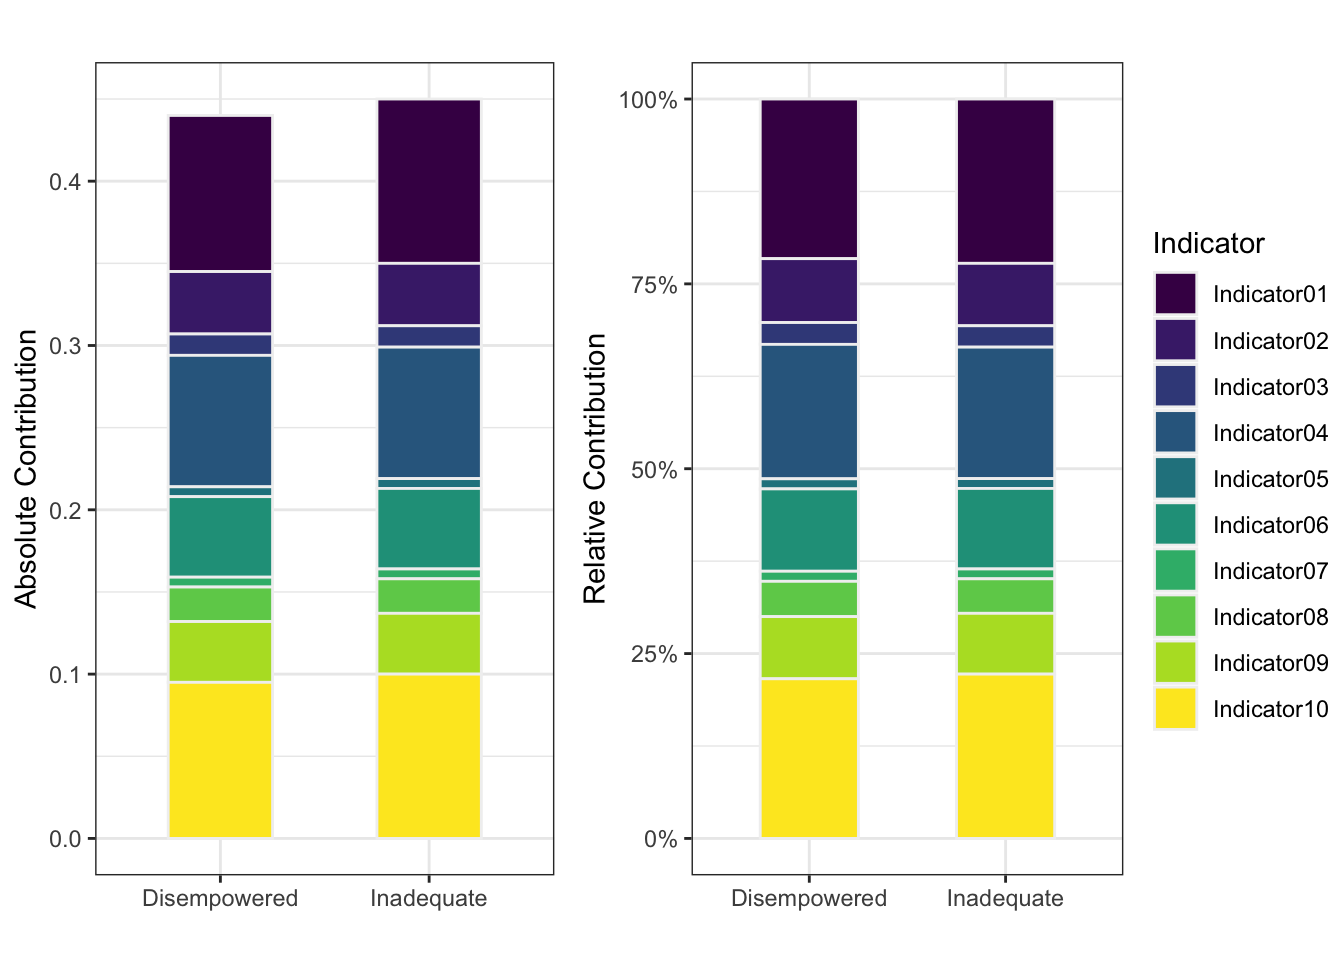
\includegraphics[width=0.8\linewidth,height=0.8\textheight]{./_figs/IDX-uncensored1-1} \end{center}

  \bibliography{book.bib,packages.bib,indexes.bib}

\end{document}
